%basic setup
\documentclass[11pt]{article}
\usepackage[margin=1in]{geometry}
\usepackage[utf8]{inputenc}
%for figures
\usepackage{float}
\usepackage{graphicx}
\usepackage{caption}
\usepackage{subfigure}
%for math environment
\usepackage{amsfonts}
\usepackage{amsmath}
\usepackage{amsthm} % for theorems, definitions
\theoremstyle{definition}
\newtheorem{definition}{Definition}[section]
\newtheorem{exmp}{Example}[section]
\usepackage{array} %for tables
\usepackage{listings}%for embedded code
\usepackage{color}
\usepackage{hyperref} %for web urls
\usepackage{siunitx} %for ohm symbol
\usepackage{diagbox} % diagonal table
\usepackage{bm} %boldsymbol

%we can define new colors to use in our report
\definecolor{mygreen}{rgb}{0,0.6,0}
\definecolor{mygray}{rgb}{0.5,0.5,0.5}
\definecolor{mymauve}{rgb}{0.58,0,0.82}

\usepackage{hyperref}

\setlength\parindent{24pt}
\lstset{ %
  frame=single,
  aboveskip=2mm,
  belowskip=2mm,
  columns=flexible,
  basicstyle={\small\ttfamily},        % size of fonts used for the code
  breaklines=true,                 % automatic line breaking only at whitespace
  captionpos=b,                    % sets the caption-position to bottom
  commentstyle=\color{mygreen},    % comment style
  escapeinside={\%*}{*)},          % if you want to add LaTeX within your code
  keywordstyle=\color{blue},       % keyword style
  stringstyle=\color{mymauve},     % string literal style
  language=python,
  numbers=left,
  stepnumber=1,
  showstringspaces=false,
  tabsize=3,
  breakatwhitespace=true,
  caption=\lstname
}
\DeclareMathOperator*{\argmax}{argmax} % thin space, limits underneath in displays
\DeclareMathOperator*{\argmin}{arg\,min}
\lstset{  
    caption=\lstname
}
\newcommand*{\oneup}{..}%

%Title of Lab
\title{ \huge{LeNet %<==replace with topic of lab
		\\ \textcolor{mygray}{\noindent\rule{12cm}{0.4pt}}
		 \\ Paper and Implementation Notes%<==replace with laboratory number
		}}
		
\begin{document} %!!!don't forget to put \end{document} at the end -> do it now!!!
\maketitle %prints your title

\vfill


\vspace{5mm}

\textbf{Erik Rosten}

\newpage


\section{Paper}

AlexNet is a paper proposed in 1998, as one of the first publications using a deep learning convolutional neural net \cite{LeNet}.

\subsection{Dataset}
LeNet is evaluated on the MNIST dataset, a subset of the NIST dataset. From the paper, it is constructed with Nist standard datasets SD-3 and SD-1. SD-1 contains 58,527 digit images by 500 different writers. SD-3 contains blocks of data from each writer in sequence. 

\bigskip

The training set is composed of the first 250 writers (around 30,000) and the rest is filled in from SD-3 to make 60,000 training samples. The test set is composed of 5,000 images from each set. 

\bigskip

The dataset was processed so they are size normalized to fit in a 20x20 pixel box while preserving aspect ratio. The resulting images contain gray levels as a result of image interpolation techniques of the normalization algorithm. They are centered by computing the center of mass of the pixels, and translating the image such that the center of mass is in the center of a 28x28 field. This is the MNIST dataset. 

\subsection{Preprocessing}

\begin{itemize}
\item White pixels scaled to -0.1
\item Black pixels scaled to 1.175
\item Makes the mean roughly 0 and the variance roughly 1
\end{itemize}

\subsection{Important Concepts}
\subsubsection{Learning from Data}
Theoretical and experimental work has shown that the gap between the expected test error and training error approximately decreases as 

\[ E_{test} - E_{train} = k \left(\frac{h}{P}\right)^{\alpha}\]

where

\begin{itemize}
\item P is the number of training samples
\item h is the "effective capacity" of the machine
\item $\alpha$ is between 0.5 and 1.0
\item k is a constant
\end{itemize}

As the capacity $h$ increases, the training error $E_{train}$ decreases, but there is a trade-off between the decrease of $E_{train}$ and the increase of the gap. There is an optimal value of $h$ that achieves the lowest generalization error $E_{test}$. Regularization (structural risk minimization) is a tool to help with this and can be implemented as minimizing

\[E_{train} + \beta H(W) \]

where H(W) is a regularization function, and $\beta$ is a constant. H(W) typically takes large values on parameters W, which limits the capacity of the accessible subset of the parameter space. 

\subsubsection{Convolutional Networks}
Convolutional Networks combine 3 ideas to ensure some degree of shift scale and distortion invariance: local receptive fields, shared weights and spatial or temporal sub-sampling.

\bigskip

Using local receptive fields, neurons can extract elementary visual features, which are then combined in subsequent layers to detect higher order features. By sharing weights among a set of units whose receptive fields are located at different places on the image, we force these feature detectors to be useful on the entire image. Each feature detector with the same weight is dubbed a feature map. A unit in a feature map that has a filter size of 5x5 would have 25 inputs, and it's receptive field would be the 5x5 area in the input. Thus, one unit has 25 trainable coefficients and 1 bias unit. The receptive fields of neighboring units in a feature map overlap int he original image, but share weights and detect the same feature at all locations in the input. Then if the image is shifted, the feature map output will be shifted by the same amount and left unchanged otherwise. This leads convolutional networks to be robust with respect to shifts and distortions of the input. 

\bigskip

Once a feature is detected, its exact location is not as important as its position in relation to other features and may in fact be harmful as the exact location with respect to different features may change depending on the image given. In terms of MNIST, the example of a horizontal line at the top and corner in the top right for a 7 is given. These locations may be different for different 7's given. To reduce the spatial resolution of the feature maps, sub-sampling layers (pooling) are formed, which reduce the resolution of the feature map and further reduce the sensitivity of the network to shifts and distortions. LeNet uses average pooling, and multiplies the result by a coefficient and adds a bias. These parameters control the effect of the sigmoid nonlinearity. If the coefficient is small, the sub-sampling layer blurs the input. If the coefficient is large, they perform a "noisy OR" or "noisy AND" depending on the bias value.  

\bigskip

In LeNet-5, the centers of the receptive fields of the last convolutional layer form a 20x20 area in the center of the input image. 


\subsection{Architecture}

\subsubsection{Activation Function}
The \textbf{sigmoid} function is used in the output layer as it accelerates training time. 

\[ S(x) = \frac{1}{1+e^{-x}} = \frac{e^{x}}{e^{x}+1}\]



\begin{figure}[H]
\begin{center}
  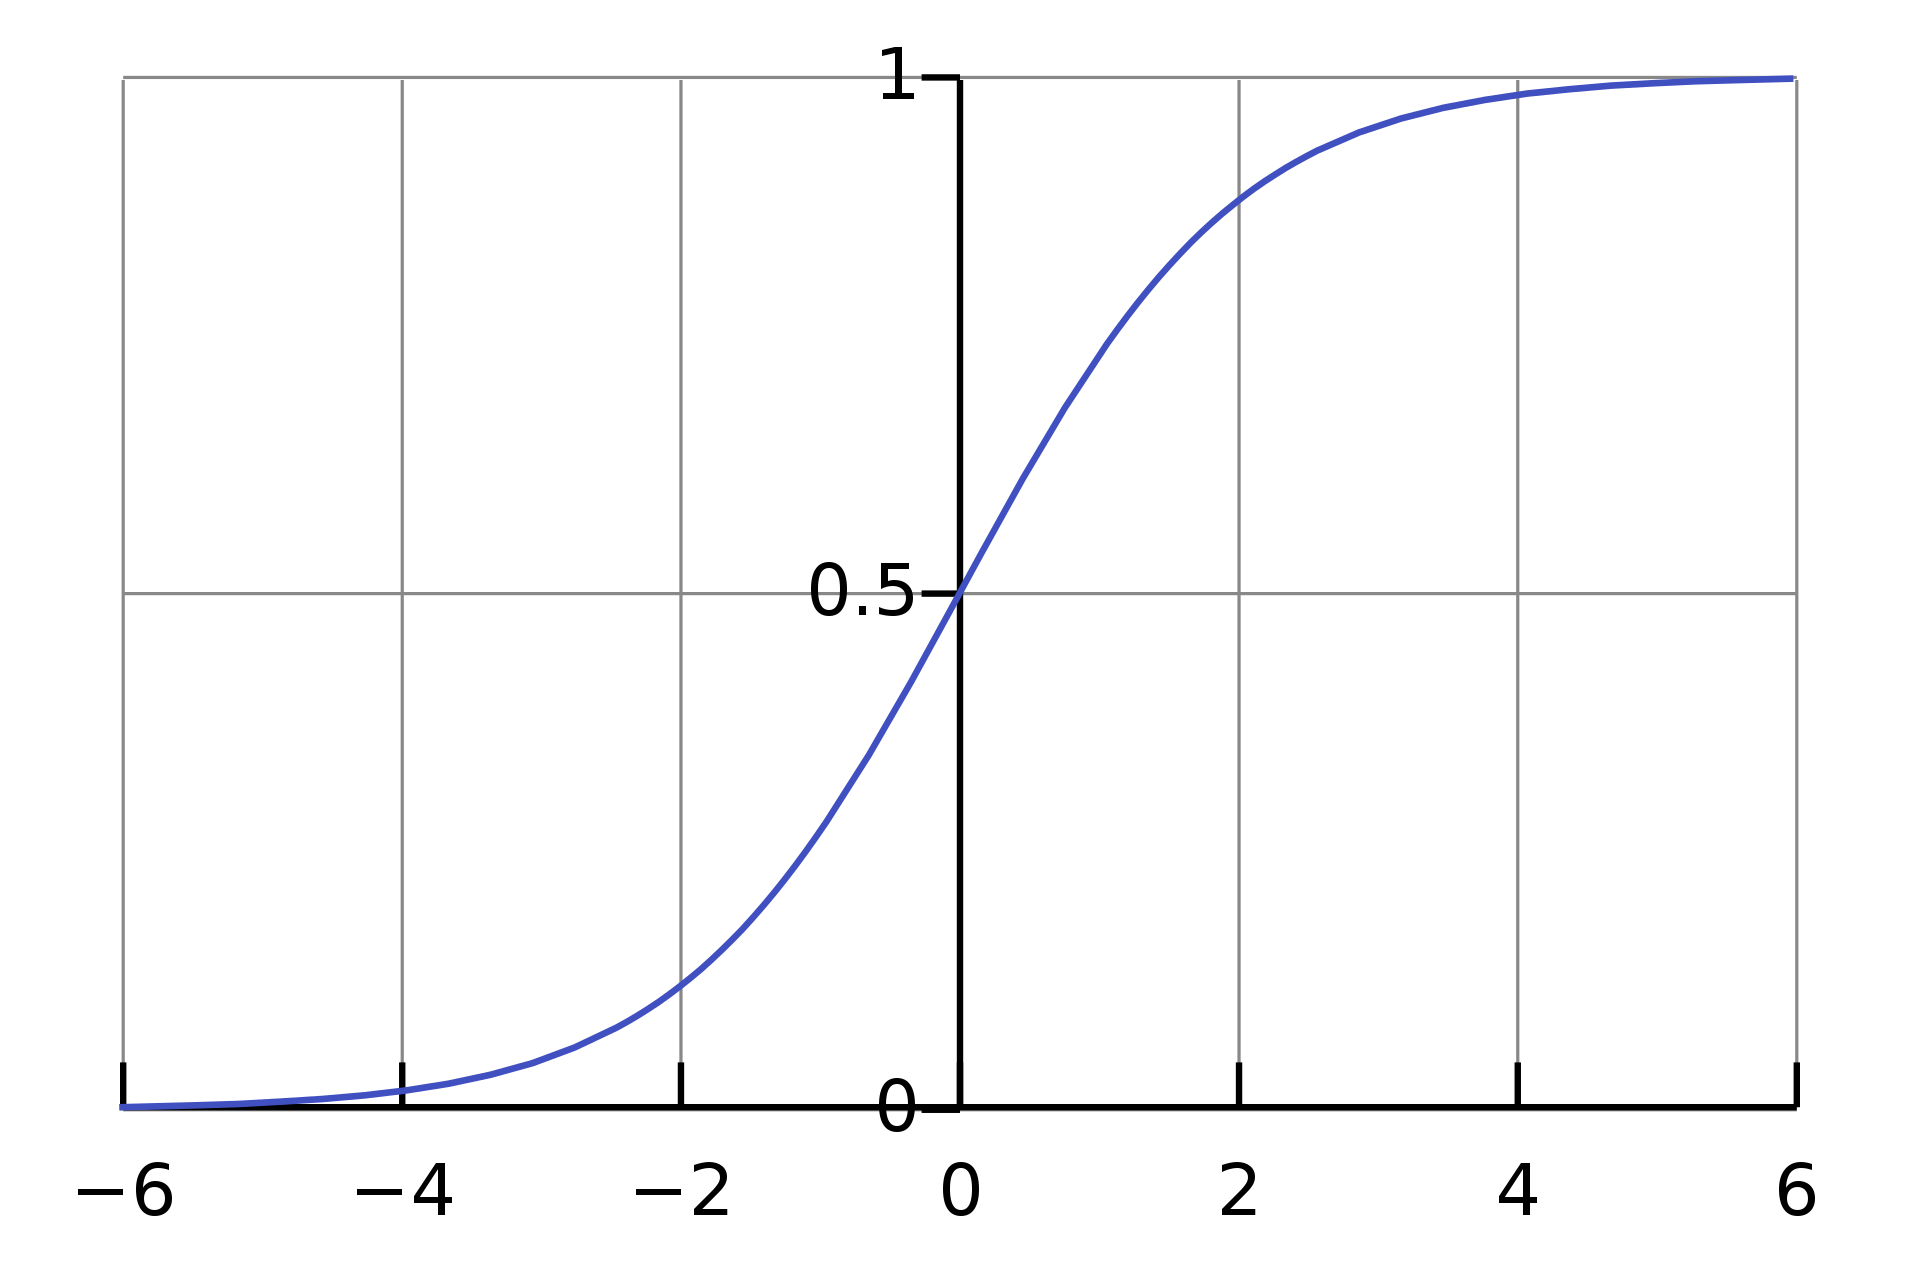
\includegraphics[width=\linewidth,keepaspectratio]{images/sigmoid.png}
  \caption{Sigmoid Function}
\end{center}
\end{figure}

The \textbf{Tanh} function is used in all other layers, which is a rescaled sigmoid function

\[ tanh(x) = 2 S(x) - 1 \]

A comparison is below where the blue is the sigmoid, and red is tanh

\begin{figure}[H]
\begin{center}
  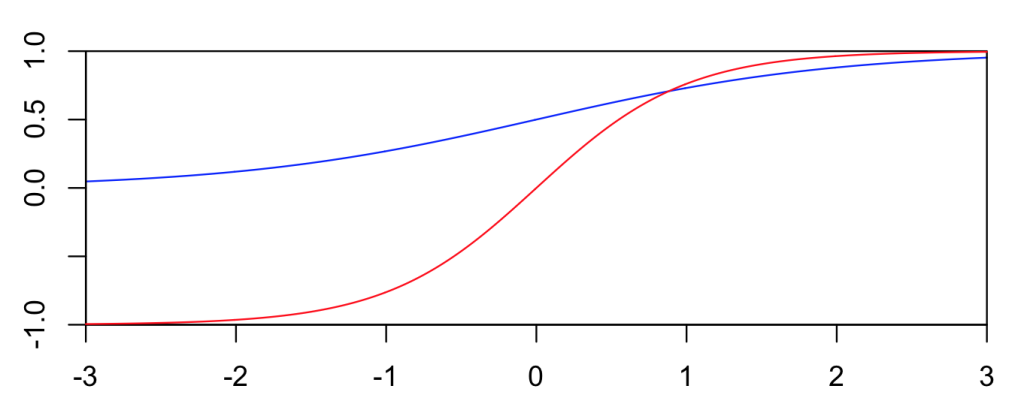
\includegraphics[width=\linewidth,keepaspectratio]{images/tanhvssigmoid.png}
  \caption{Tanh vs Sigmoid Functions}
\end{center}
\end{figure}

ReLU was not available at the time of the publishing of the paper. 

\subsubsection{Final Architecture}




Resulting image size is calculated as 

\begin{equation}
 ceil\left(\frac{W-K+2P}{S}\right) + 1
 \end{equation}

where

\begin{itemize}
\item W is the input width
\item K is the kernel size
\item P is the padding
\item S is the stride
\end{itemize}

Trainable parameter calcluations from convolutional layers can be calculated as

\[ f \cdot K^{2} \cdot C\]

where K is the kernel size, f is the number of feature maps of that layer, and C is the number of channels in the previous layer

\bigskip 

Trainable parameters calculations from fully connected layers can be calculated as 

\[ C_{in} \cdot C_{out}\]

where $C$ represents number of input and output channels. 


\begin{table}[H]
\centering
\begin{tabular}{| c | c | c | c | c | c |}
\hline
Layer Name & Feature Maps & Kernel Size & Stride & Resulting Image Size &  Trainable Parameters\\
\hline
Conv1 & 6 & 5 x 5 & 1 & 28 x 28 x 6 & 156\\
\hline
Average Pooling & 6 & 2 & 2 & 14 x 14 x 6 & 12\\
\hline
Conv2 & 16 & 5 x 5& 1 & 10 x 10 x 16 & 1,516**\\
\hline
Max Pooling & 16 & 2 & 2 & 5 x 5 x 16 & 32 \\
\hline
Conv3 & 120 & 5 x 5 & 1 & 1 x 1 x 120 & 48,120 \\
\hline
FC1 & -  &  - &  - & 84 & 10,164 \\
\hline
RBF Output Layer & - & - & - & - & - \\
\hline
Total & - & - & - & - & 60,000 \\
\hline
\end{tabular}
\caption{Summary of LeNet-5}
\end{table}

** The second convolutional layer combines different pooling feature maps in a different scheme. The table below shows this scheme
\begin{figure}[H]
\begin{center}
  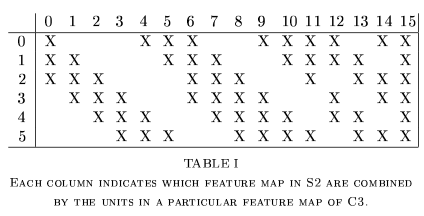
\includegraphics[width=\linewidth,keepaspectratio]{images/S2C3.png}
\end{center}
\end{figure}

Thus, the number of trainable parameters as usually computed assumes all input feature maps are mapped to each output feature map. However, here we have that the 1st feature map of C3 connects 3 feature maps of S2. Then, for this particular connection we have

\[ 5 \cdot 5 \cdot 3 = 75 + 1 = 76 \; \; \text{Trainable Parameters} \]

where the 3 comes from the bias. We have 76 trainable parameters for each C3 feature maps 0,1,2,3,4,5.

There are 4 S2 feature maps in C3 feature maps 6,7,8,9,10,11,12,13,14 with $100 + 1$ trainable parameters each. Finally, there are 6 S2 feature maps in C3 feature map 15 giving $151$ trainable parameters.

Then, the total number of trainable parameters for this layer are 

\[ (76 \cdot 6) + (101 \cdot 9) + (151 \cdot 1) = 1516 \; \; \text{Trainable Parameters}\]

\bigskip

This type of connection scheme is unusual in todays CNN's, but was motivated in the paper as forcing the symmetry in the network to be broken and forcing different C3 feature maps to extract different complementary features. It had the added benefit of reducing the number of connections and trainable parameters. Using the more common fully connected scheme results in 

\[ (5 \cdot 5 \cdot 6 + 1) \cdot 16 = 2416 \; \; \text{Trainable Parameters}\]

\newpage
\section{Implementation}

The implementation of LeNet5 differs from the paper in several ways summarized below
\begin{itemize}
\item The connections for C3 use the more common fully connected scheme.
\item Max Pooling instead of average pooling
\item ReLU instead of tanh/sigmoid
\item A fully connected into softmax output layer is used instead of the RBF's in the original paper
\end{itemize}

\subsection{MNIST Training}

As a baseline, we use cross entropy loss with vanilla stochastic gradient descent of learning rate 1 and train for 30 epochs.




\begin{table}[H]
\centering
\begin{tabular}{| c | c | c | c | c | c |}
\hline
Optimizer & Total Epochs & Training Accuracy & Test Accuracy & Experiment \#\\
\hline
Vanilla SGD & 30 & 87.04 & 88.23  & 1\\
\hline
SGD w/ Classic Momentum & 30 & 93.43 & 93.78 & 2 \\
\hline
SGD w/ Nesterov Momentum & 30 & 93.99 & 94.49 & 3 \\
\hline
Adam & 30 &  97.02 & 97.36 & 4 \\
\hline
Adam & 60 & 98.49 & 98.58 & 5\\
\hline
Adam & 100 & 99.08 & 98.99 & 6\\
\hline
\end{tabular}
\caption{Training Results with Different Optimizers}
\end{table}

Training plots for the last 100 epoch run of Adam are shown below
\begin{figure}[H]
\begin{center}
  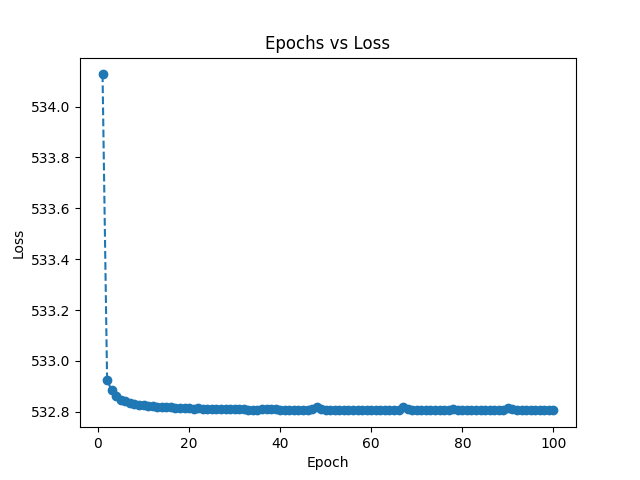
\includegraphics[width=9cm,keepaspectratio]{images/loss.png}
\end{center}
\end{figure}

\begin{figure}[H]
\begin{center}
  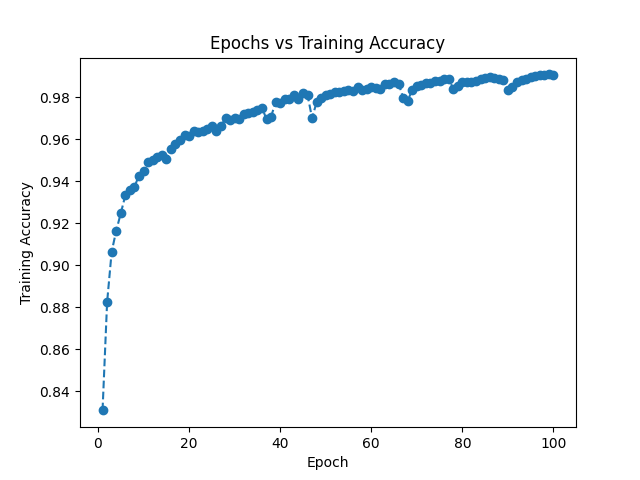
\includegraphics[width=9cm,keepaspectratio]{images/train_acc.png}
\end{center}
\end{figure}

\begin{figure}[H]
\begin{center}
  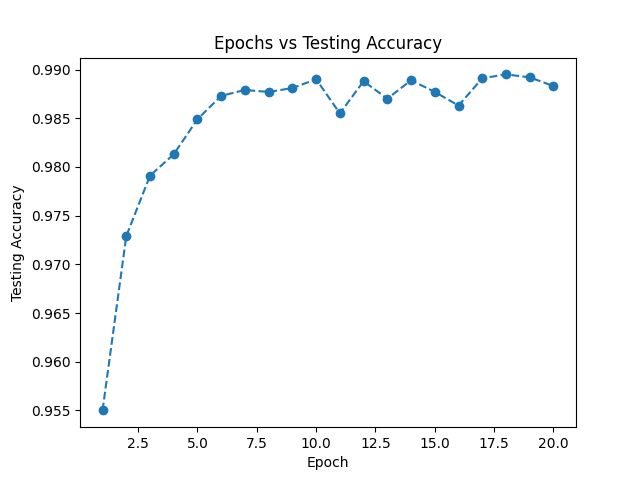
\includegraphics[width=9cm,keepaspectratio]{images/test_acc.png}
\end{center}
\end{figure}


\subsection{Testing}

I test the trained model with my own handwritten digits, and the results are shown below. The trained model correctly predicted 8/10 of my handwritten digits, misclassifying '3' as '5' and '7' as '3'. Both these misclassifications are relatively understandable, and the original paper actually shows examples of missclassification where many of them misclassify '3' as '5'.


\begin{figure}[H]
\begin{center}
  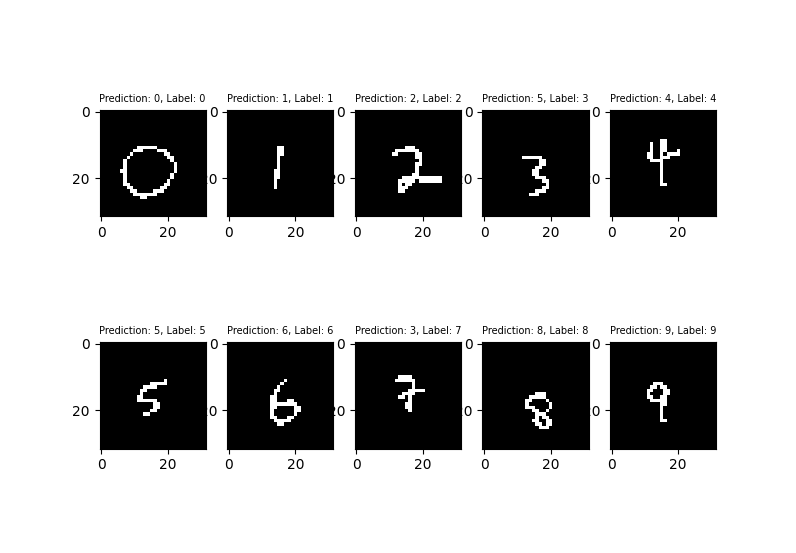
\includegraphics[width=\linewidth,keepaspectratio]{images/my_results.png}
\end{center}
\end{figure}


\newpage
\begin{thebibliography}{999}

\bibitem{LeNet}
  \emph{LeCun, Yann, Leon Bottou, Yoshua Bengio, and Patrick Haffner. “Gradient-Based Learning Applied to Document Recognition,” n.d.}.

	
\end{thebibliography}

\newpage
\section*{Code}


%\lstinputlisting[language=Python]{\oneup/Code/datagen.py}
%\lstinputlisting[language=Python]{\oneup/Code/generate_higher_dim_data.py}
%\lstinputlisting[language=Python]{\oneup/Code/generate_sample_data.py}
%\lstinputlisting[language=Python]{\oneup/Code/generate_higher_dim_data.py}
%\lstinputlisting[language=Python]{\oneup/Code/generate_sparse_data.py}
%\lstinputlisting[language=Python]{\oneup/Code/config.py}
%
%\lstinputlisting[language=Python]{\oneup/Code/part_1_pca.py}
%\lstinputlisting[language=Python]{\oneup/Code/part_2_random_projections_compressive_sensing.py}
%
%\lstinputlisting[language=Python]{\oneup/Code/part_3_sketching.py}


\end{document}